\section{Design architetturale}
%Design architetturale (architettura complessiva, descrizione di pattern architetturali usati, componenti del sistema distribuito, scelte tecnologiche cruciali ai fini architetturali -- corredato da pochi ma efficaci diagrammi)

Di seguito vengono analizzate l'architettura complessiva dell'applicazione e le decisioni critiche riguardanti pattern architetturali e tecnologie rilevanti.
Prima di pensare a qualsiasi architettura per il gioco da realizzare, ciò che si è cercato di fare è stato individuare l'engine ideale per il progetto. 
La scelta è ricaduta su Indigo in quanto: 
\begin{itemize}
    \item E' un framework specifico per il game development
    \item E' scritto in Scala 3 e favorisce lo sviluppo tramite paradigma funzionale con un approccio unidirezionale ed immutabile al flusso di dati
    \item Permette il gioco su browser, come da requisito di business, mediante compilazione tramite Scala.js.
\end{itemize}
I concetti chiave di Indigo che ci guidano nello sviluppo del gioco sono 
\begin{itemize}
    \item Paradigma Model, View, ViewModel
    \item Game loop con modello ad eventi
    \item Scene
\end{itemize}

\subsection{Paradigma Model-View-ViewModel}
Il pattern architetturale \textbf{MVVM} (Model, View, ViewModel) è una variante del famoso MVC. 
Obiettivo di questo pattern è quello di separare il modello dei dati dalla sua rappresentazione, tenendo entrambi puri e funzionali al loro scopo, frapponendo tra loro un elemento "ibrido", il ViewModel.
Di seguito l'interpretazione sulla quale si basa Indigo e che seguiamo per lo sviluppo del nostro gioco.


\begin{figure}[!hbt]
    \centering
    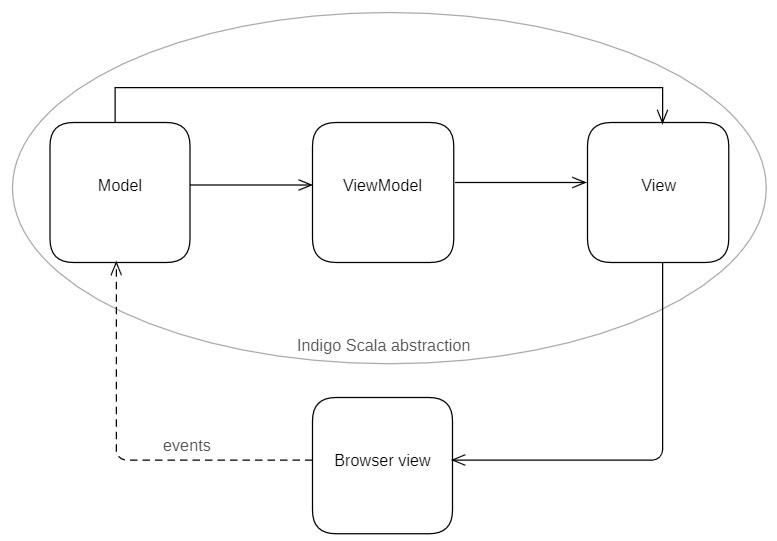
\includegraphics[scale=0.5]{mvvm.jpg}
    \caption{\textit{Architettura Model, View, ViewModel}} 
\end{figure}

\paragraph{Model}
Rappresenta il modello di gioco puro, indipendentemente dalla sua rappresentazione visuale. 
Esso contiene lo stato del gioco e la sua logica. 

\paragraph{ViewModel}
Si interpone tra Model e View. Ha lo scopo di mantenere alcuni dati utili per la rappresentazione che tuttavia non concernono la logica di gioco, devono perciò rimanere separati e non essere inclusi all'interno del Model.

\paragraph{View}
Si occupa di offrire una rappresentazione del Model e del ViewModel a schermo. Costituisce quindi la logica di visualizzazione di questi, senza contenere però alcuno stato o logica di gioco.

\subsection{Game loop con modello ad eventi}
La logica di Indigo si basa su un game loop che processa, ad ogni iterazione, una coda di eventi. 
Ad ogni ciclo, il framework esegue le seguenti operazioni:
\begin{itemize}
    \item Aggiunta dell'evento FrameTick alla coda eventi
    \item Per ogni evento, update del Model
    \item Per ogni evento, update del ViewModel
    \item Presentazione e rendering degli elementi a video
    \item Reset della coda di eventi
\end{itemize}

Il concetto di \textbf{immutabilità}, presente nel paradigma funzionale, qui si traduce non in un update di uno stato interno del modello, ma bensì nella generazione di un nuovo modello aggiornato. 

Durante l'update del Model è possibile generare eventi custom che verranno processati all'iterazione successiva. 

\subsection{Scene}
Le scene sono un modo di organizzare il codice secondo una logica di gioco ben definita. Sono un meccanismo di suddivisione che permette di individuare delle "fasi" di gioco da sviluppare in modo separato le une dalle altre.
In ogni istante all'interno del gioco la scena indicata come "corrente" è abilitata all'aggiornamento del Model/ViewModel, alla gestione degli eventi in coda ed infine alla presentazione a schermo: la scena corrente può leggere e aggiornare solo i suoi dati che sono un sottoinsieme di quelli globali. 

Abbiamo identificato quattro scene principali su cui andare a definire Lost 'n Souls. 

\begin{figure}[!hbt]
    \centering
    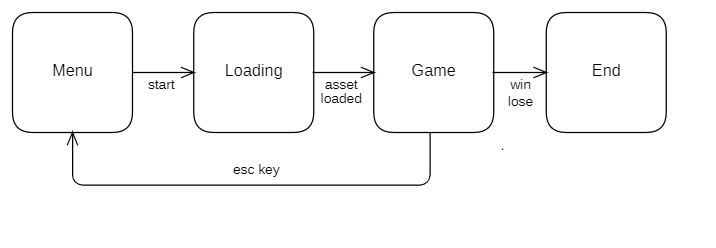
\includegraphics[scale=0.75]{scenes.jpg}
    \caption{\textit{Il flusso delle scene}}
\end{figure}

\subsection{Architettutra di Model e ViewModel}

Come conseguenza della suddivisione di cui sopra, il Model principale è costituito dai singoli Model relativi a ciascuna scena. Stessa cosa vale per il ViewModel. 

Da notare che una scena, per la sua presentazione a video, può non necessitare di un Model o di un ViewModel, lo stesso concetto si può estendere per una View qualsiasi la quale potrebbe basarsi solo su Model.

\begin{figure}[!hbt]
    \centering
    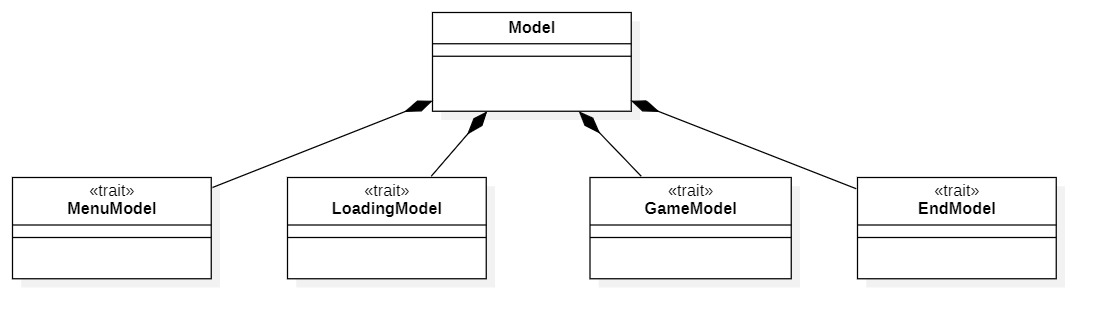
\includegraphics[scale=0.45]{model.jpg}
    \caption{\textit{Il Model}} 
\end{figure}

\newpage 
\subsection{Elementi principali del GameModel}
All'interno della scena di gioco, abbiamo identificato i principali componenti:

\begin{itemize}
    \item \textbf{Character} Personaggio controllato dal giocatore
    \item \textbf{Dungeon} Intera mappa di gioco nel suo complesso
    \item \textbf{Room} Stanza situata all'interno di una mappa di gioco
    \item \textbf{Anything} Una qualsiasi entità da visualizzare all'interno di una stanza: nemico, oggetto, elemento bloccante o anche lo stesso Character. 
    
\end{itemize}


\begin{figure}[!hbt]
    \centering
    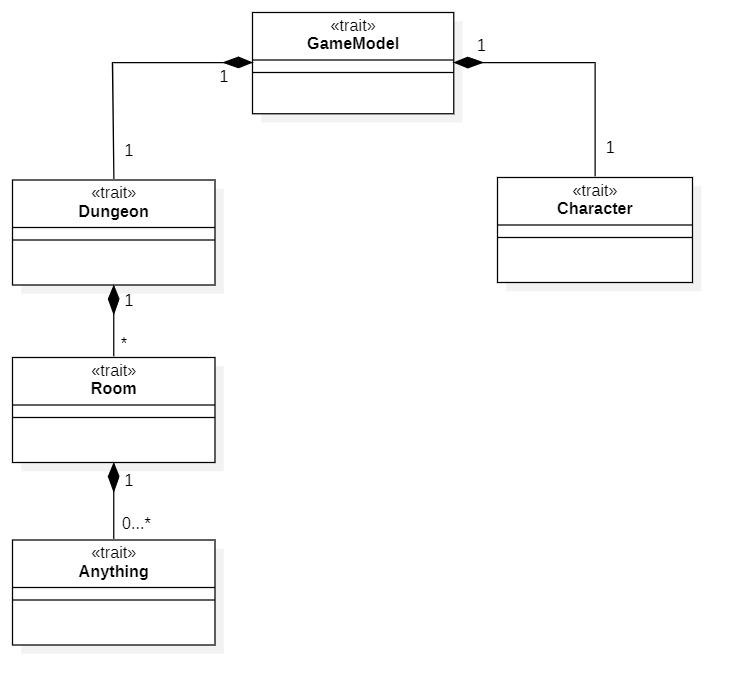
\includegraphics[scale=0.5]{gamemodel.jpg}
    \caption{\textit{Diagramma degli elementi principali del GameModel}} 
\end{figure}